\section{Theorie}
Der Germanium-Detektor wird zur $\gamma$-Spektroskopie verwendet, da dieser
gegenüber eines Szintillations-Detektors eine viel höhere Auflösung besitzt.

\subsection{Wechselwirkung von Gamma-Strahlung mit Materie}
Da die $\gamma$-Quanten in dem Detektor mit der Materie wechselwirken, werden
zunächst die Wechselwirkungen näher erläutert:

\begin{itemize}
  \item Bei dem \textbf{Photoeffekt} gibt das $\gamma$-Quant die komplette Energie
  an ein Hüllenelektron (meist aus der K-Schale) des Atoms ab. Übersteigt diese
  Energie die Bindungsenergie des Elektrons, so wird dieses aus dem Atom
  herausgelöst. Die übrige Energie erhält das Elektron als kinetische Energie.
  Da bei dem Herauslösen des Elektrons ein Loch entsteht, wird dieses durch ein
  anderes Elektron einer höheren Schale aufgefüllt, dabei wird Energie in Form
  von $\gamma$-Strahlung frei, welches ein weiteres Elektron aus einer höheren
  Schale herauslösen kann. Dieses zweite herausgelöste Elektron wird Auger-Elektron
  genannt.
  Der Wirkungsquerschnitt $\sigma_{\symup{Ph}}$ für den Photoeffekt ist stark
  abhängig von der Energie der $\gamma$-Quanten und der Kernladungszahl des
  Materials:
  \begin{equation}
    \sigma_{\symup{Ph}} \propto Z^{\alpha}E^{\delta}
  \end{equation}
  wobei die Exponenten empirisch festegestellt wurden mit $4<\alpha<5$ und
  $\delta \approx -3,5$. $\delta$ kann aber für Energien ab \SI{5}{\mega\eV} auf
  einen Wert bis zu -1 steigen.

  \item Eine weitere wichtige Wechselwirkung ist der \textbf{Compton-Effekt}.
  Hierbei streut das $\gamma$-Quant elastisch an einem freien Elektron und gibt
  Teil seiner Energie an dieses in Form von kinetischer Energie ab.
  Die Streuung bewirkt eine Energieabnahme und Richtungsänderung des
  $\gamma$-Quants, wobei ein maximaler Energieübertrag bei einer Richtungsänderung
  von $\Psi_{\gamma} = \pi$ stattfindet:
  \begin{equation}
    E_{\gamma}' = E_{\gamma} \cdot ( 1+\epsilon(1-\cos{\Psi_{\gamma}}))^{-1} \;
    \symup{mit} \; \epsilon = \frac{E_{\gamma}}{m_0c²}
  \end{equation}
  Die Herleitung des Wirkungsquerschnitts $\sigma_{\symup{Co}}$ für den Compton-Effekt
  ist sehr lang und kompliziert und wird deswegen hier nicht weiter erläutert.
  Aus dieser Herleitung folgt:
  \begin{equation}
    \sigma_{\symup{Co}}=\frac{3}{4}\sigma_{\symup{Th}}
    \left( \frac{1+\epsilon}{\epsilon^2} \left[ \frac{2+2\epsilon}{1+2\epsilon} -
    \frac{1}{\epsilon} \ln{(1+2\epsilon)} \right] +
    \frac{1}{2\epsilon}\ln{(1+2\epsilon)} -
    \frac{1+3\epsilon}{(1-2\epsilon)^2}\right)
  \end{equation}
  mit
  \begin{equation}
    \sigma_{\symup{Th}} = \frac{8}{3}\pi \left(\frac{e_0}{4 \pi \epsilon_0 c^2 m_o} \right)^2
    := \frac{8}{3}\pi r_e^2
  \end{equation}
  wobei $e_o$ die Elementarladung, $c$ die Vakuumlichtgeschwindigkeit,
  $\epsilon_0$ die Influenzkonstante, $m_0$ die Masse eines Elektrons und
  $r_e$ den klassischen Elektronenradius darstellt.

  \item Bei der \textbf{Paarerzeugung} stößt ein $\gamma$-Quant mit einem
  Stoßpartner zusammen, wobei ein Elektron und ein Positron erzeugt wird.
  Bei einem Atom als Stoßpartner muss die Energie des $\gamma$-Quants
  mindestens gleich der Ruheenergie von einem Elektron und einem Postiron sein,
  da hierbei die Energie in Masse umgewandelt wird. Der Impuls wird hierbei
  an das Atom weitergegeben. Bei einem Elektron als Stoßpartner muss das
  $\gamma$-Quant mindestens die vierfache Ruheenergie eines Elektrons besitzen,
  da hier der Impuls nicht komplett an das Stoßelektron übergeben werden kann,
  aufgrund der geringen Masse des Elektrons.
  Der Wirkungsquerschnitt $\sigma_{\symup{Pa}}$ der Paarerzeugung kann mit viel
  Aufwand hergeleitet werden. Hier sind nur die Ergebnisse dargestellt, wobei
  unterschieden werden muss für kernnahe und kernferne Paarbildung.
  Für die kernnahe Paarbildung, also Bereiche von 10-15\,\si{\mega\eV}, gilt
  die folgende Gleichung:
  \begin{equation*}
     \sigma_{\symup{Pa}}= \alpha r_e^2z^2 \left( \frac{28}{9} \ln{2 \epsilon} -
     \frac{218}{27} \right)
  \end{equation*}
  Für die kernferne Paarbildung (außerhalb der Elektronenhülle) lässt sich der
  Wirkungsquerschnitt wie folgt berechnen:
  \begin{equation}
    \sigma_{\symup{Pa}}= \alpha r_e^2z^2 \left( \frac{28}{9} \ln{\frac{183}{\sqrt[3]{z}}} -
    \frac{2}{27} \right)
  \end{equation}
\end{itemize}
In Abbildung \ref{abb:1} sind die Intensitäten der Wechselwirkungen gegen die
Energie der $\gamma$-Quanten aufgetragen.

\begin{figure}
  \centering
  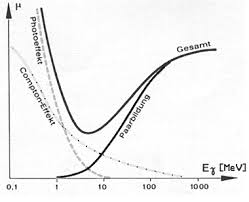
\includegraphics[scale=0.8]{Wechselwirkung.jpeg}
  \caption{Intensitäten der Wechselwirkungen. \cite{Q2}}
  \label{abb:1}
\end{figure}

\subsection{Aufbau und Wirkungsweise eines Germanium-Detektors}
Der Halbleiter-Detektor besteht im Wesentlichen aus einer Halbleiterdiode,
welche aus zwei Schichten besteht: Der n-dotierten Schicht, als
Elektronen-Donator, und einer p-dortierten Schicht, als Elektronen-Akzeptor.
In dem Bereich zwischen den beiden Schichten entsteht eine Sperrschicht, durch
Rekombination der Löcher aus der p-Schicht und den Elektronen aus der n-Schicht.
Die benannten Löcher sind Elektronenlöcher, welche hier wie positiv geladene
Teilchen angesehen werden können.
Diese Sperrschicht ist wichtig für die Funktionsweise eines Germaniumdetektors,
da hier die Wechselwirkung zwischen den Photonen und der Materie stattfindet, bzw.
nur hier die Wechselwirkung zu einem Zählereignis führt.
In der Sperrschicht werden Elektronen durch die vorher benannten Wechselwirkungen
mit sehr hohen kinetischen Energien freigesetzt. Diese widerum regen andere
Elektronen an, die zwar geringere kinetische Energien haben, aber genug um die
Lücke zwischen dem Leitungsband und dem Valenzband zu überspringen. So
entstehen in der Sperrschicht bzw. ladungsträgerarmen Zone Löcher und Elektronen,
die durch eine außen anliegende Spannung getrennt werden können, ohne wieder zu
rekombinieren. Durch diesen Vorgang entsteht ein Stromfluss, welcher zu einem
Zählereignis führt.
Um ein möglichst genaues Messergebnis zu erhalten, ist es sinnvoll die
ladungsträgerarme Zone zu verbreitern, denn die Breite beträgt ohne äußere Einflüsse
nur einige \si{\micro\meter}, da nur in diesem Bereich Photonen detektiert werden
können. Eine hohe außen angelegte Spannung (einige \si{\kilo\volt}), vergrößert
die ladungsträgerarme Zone auf einige \si{\centi\meter}, dies ist nur begrenzt
möglich, da sich die Halbleiterdiode durch die hohe Spannung erhitzt und somit
thermische Elektronen freigesetzt werden, die somit auch in das Leitungsband
übergehen können und somit für einen Strom sorgen, der die Messergebnisse
verfälscht. Deswegen wird während der Messung der Germaniumkristall mit
flüssigem Stickstoff auf $\SI{77}{\kelvin}$ gekühlt.
Außerdem ist die Dicke $d$ der Sperrschicht abhängig von der Dotierung
der Schichten, wie in Gleichung \eqref{eq:1} zu sehen.

\begin{equation}
  \label{eq:1}
  d = d_p + d_n \approx d_p \approx \sqrt{\frac{2 \epsilon \epsilon_0}
  {e_0}(U_D+U) \frac{1}{n_A}}
\end{equation}
Um die Dicke also zu vergrößern ist es sinnvoll die Akzeptorendichte $n_A$ so
gering wie möglich zu halten, deswegen wird für einen Germaniumdetektor ein
sehr reiner Germanium-Kristall mit $n_A \approx 10^{10}\,
\frac{\symup{Atome}}{\symup{cm}} $.

Der schematische Aufbau eines Germanium-Detektors ist in Abbildung \ref{abb:3}
zu sehen.

\begin{figure}
  \centering
  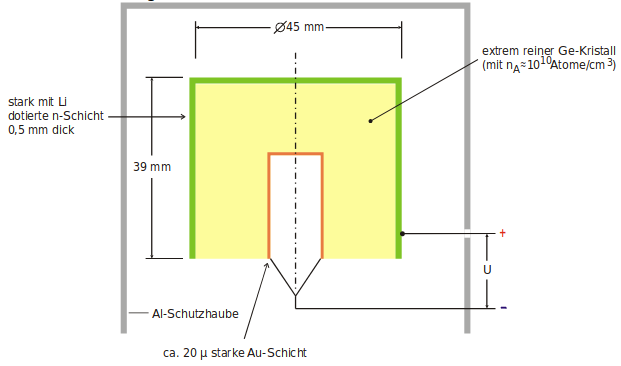
\includegraphics[scale=0.5]{AufbauDetektor.png}
  \caption{Schematischer Aufbau eines Germanium-Detektors. \cite{Q1}}
  \label{abb:3}
\end{figure}

Als p-dotierte Schicht wird der sehr reine Germaniumkristall genommen und als
n-Schicht eine sehr dünne Lithiumschicht. Eine zusätzliche leitfähige
Goldschicht wird im inneren des Kristalls aufgetragen, um als Anschluss für
die Gleichspannung zu dienen. Der Detektor ist außerdem mit einer Aluminium
Schutzhaube umgeben. Zusätzlich wird die natürliche Untergrundstrahlung durch
eine Blei-Schicht abgeschrimt, um die Messergebnisse nicht zu verfälschen.
Um gegebenenfalls strahlende Isotope aus dem Blei abzuschirmen, wird noch eine
weiter Schicht aus Kupfer unter der Blei-Schicht angebracht.

\subsection{Energiespektrum}
In Abbildung \ref{abb:4} ist das Energiespektrum eines monochromatischen
$\gamma$-Strahlers zu sehen.
\begin{itemize}
  \item Der \textbf{Photopeak} ensteht durch vollständige Abgabe der Enerige
  durch den Photoeffekt.
  \item Das \textbf{Compton-Kontinuum} wird die Comptonstreuung hervorgerufen,
  hierbei wird nur ein Teil der Energie abgegeben, deswegen ist dies für die
  Energiebestimmung des Photons nicht nützlich. Die Comptonkante entsteht durch
  den maximalen Energieübertrag bei einer Richtungsänderung des Photons von 2\pi.
  Nach der Compton-Kante ist dennoch eine Intensität zu erkennen, dieser kommt
  durch mehrfach compton-gestreute Photonen zustande.
  \item Der \textbf{Rückstreupeak} ensteht auch durch Comptonstreuung, aber
  nicht in dem Detektor, sondern in der Umgebung, beispielsweise in der
  Abschirmung.
\end{itemize}

\begin{figure}
  \centering
  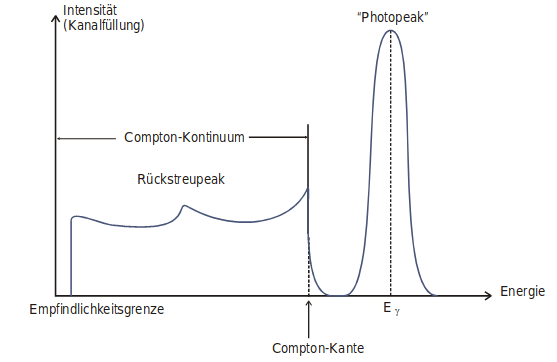
\includegraphics[scale=0.5]{Spektrum.png}
  \caption{Spektrum eines monochromatischen $\gamma$-Strahlers. \cite{Q1}}
  \label{abb:4}
\end{figure}

\subsection{Energetisches Auflösungsvermögen und Effizienz}
Eine Kenngröße des Halbleiter-Detektors ist das energetische Auflösungsvermögen.
Als Maß hierfür die Halbwertsbreite des Photopeaks angegeben (bei
monochromatischer \gamma-Strahlung). Diese ist vor allem abhängig von der
Anzahl der Elektronenlochpaare.
Durch einige Einfüsse wird das energetische Auflösungsvermögen dennoch vermindert:
\begin{itemize}
  \item Rauschen des Leckstroms, durch Eigenleitung und Restverunreinigung.
  Dies wird durch Abkühlen der Aperatur verringert.
  \item Rauschen des Verstärkers
  \item unvollständige Ladungssammlung durch Feldinhomogenitäten
\end{itemize}
Die Effizienz bezeichnet die Energieabhängigkeit der Nachweiswahrscheinlichkeit
bei der Detektion von Photonen.

\subsection{Aufbau}

Der Aufbau des Versuchs ist in Abbildung \ref{abb:2} zu sehen. Folgende
Komponenten sind in dem Aufbau enthalten:
\begin{itemize}
  \item \textbf{Detektor}: Zur Detektion der $\gamma$-Strahlen mit Hilfe
  einer Halbleiterdiode.
  \item \textbf{Vorverstärker}: Der Vorverstärker integriert die vom Detektor
  kommende Ladungsmenge in einen Spannungsimpuls, da Spannung mit geringeren
  Verlusten weitergeleitet werden kann als Strom. Damit durch die Integration
  theoretisch keine unendlich hohe Spannung ensteht, muss der Kondensator am
  Vorverstärker nach jedem Ladungsimpuls entladen werden. Da durch eine
  Entladung über einen Widerstand ein Rauschen entsteht, wird der Kondensator
  durch eine optoelektrische Rückkopplung entladen, bei der die Gate-Drain-Schicht
  des Operationsverstärkers mit einer LED beleuchtet wird, wobei die
  Sperrschicht kurz leitend wird und die LAdung somit abfließen kann.
  \item \textbf{Hauptverstärker}: Der Hauptverstärker verstärkt die Spannung
  nach dem Vorverstärker. Wobei darauf geachtet werden muss, dass die Bandbreite
  des Operationsverstärkers weder zu klein noch zu groß ist, um alle Signale zu
  übertragen und das Rauschen nicht zu groß werden zu lassen.
  Zusätzlich differenziert und integriert der Hauptverstärker, als Hoch- und
  Tiefpassfilter.
  \item \textbf{Vielkanalanalysator}: Im Vielkanalanalysator sortiert
  die Spannungsimpulse nach ihrer Größe und zählt diese, indem ein Kondensator
  durch den zu messenden Spannungsimpuls geladen wird und die Zeit der
  Entladung erfasst wird. Der Kondensator ist zusätzlich an eine
  Gleichspannungsquelle angeschlossen. Da die Entladezeit ein Maß für die
  Höhe des Spannungsimpulses ist, wird die Zählerstelle des zur Entladezeit
  passenden Kanals um eins erhöht. Zur Messzeit wird das Gatter zu dem Kondensator
  geschlossen, damit kein zweiter Spannungsimpuls während der Messung
  den Kondensator auflädt und somit die Messung verfälscht.
  Die Messungen des Vielkanalanalysators werden auf dem angeschlossenen
  Computer gespeichert.
  \item \textbf{Temperaturregler}: Während der Messung wird die Aperatur
  durchgehgend durch flüssigen Stickstoff gekühlt, aufgrund der oben genannten
  Störstellen.
\end{itemize}

Um keine Verstärkung von Gleichspannungen und Offsetspannungen zu erhalten, wird
zwischen dem Vorverstärker und dem Hauptverstärker ein RC-Glied geschaltet. Ein
unerwünschter Nebeneffekt sind Unterschwingungen, welche zur Verschlechterung
des 1auflösungsvermögen führen. Um dies zu vermeiden wird ein Teil der
Gleichspannung über das RC-Glied geleitet ("Pole-Zero-Kompensation"). Das gleiche
Verfahren wird am Ausgang des Hauptverstärkers durchgeführt
("Base-Line-Restorer").

\begin{figure}
  \centering
  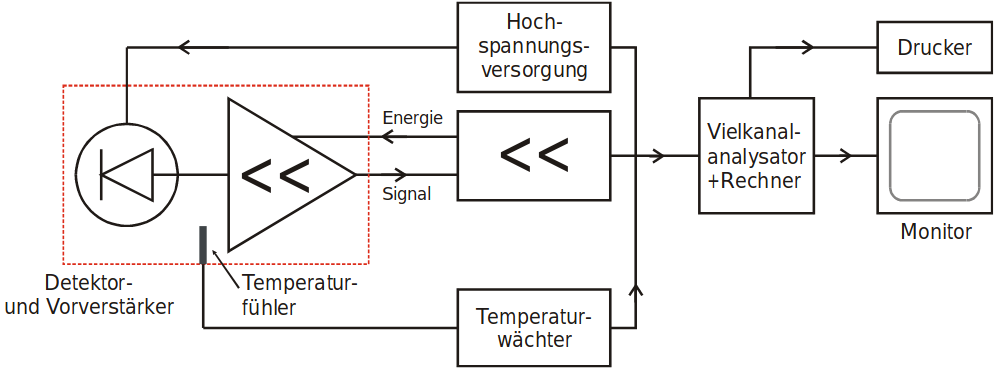
\includegraphics[scale=0.4]{Aufbau.png}
  \caption{Versuchsaufbau. \cite{Q1}}
  \label{abb:2}
\end{figure}



\section{Durchführung}
Zur Durchführung des Versuches wird zunächst die Gleichspannung langsam auf \SI{5}{\kilo\volt}
erhöht.
Die Probe und der Detektor befinden sich in einem mit Blei abgeschirmten Kasten,
um die Hintergrundstrahlung abzuschirmen. Außerdem ist die Bleischicht im Inneren
noch zusätzlich mit einer Kupferschicht umgeben, um gegebenenfalls strahlende
Blei-Isotope aus der Bleischicht abzuschirmen.
Nacheinander werden die jeweiligen Proben mit Hilfe eines Abstandhalters
vor dem Detektor befestigt. Die Messung wird für jede Probe je eine Stunde lang
durchgeführt.
